\subsection{An oriented complex-character example}

The numerical illustration uses three primitive characters modulo $5$:
the quartic character $\chi(2)=i$, its conjugate, and its quadratic
square. Direct evaluation uses the finite Hurwitz-zeta identity
\[
 L(s,\chi)=5^{-s}\sum_{a=1}^4\chi(a)\zeta(s,a/5).
\]
The functional equation supplies a real Hardy normalization on the
critical line. A sign-change scan on $[-40,40]$ followed by
high-precision root refinement detected $31$ ordinates for the
quartic character and $32$ for its square. The quartic list has $16$
negative and $15$ positive entries; its conjugate's list is its
reflection. Reevaluating the saved decimal ordinates at $80$-digit
precision gives direct $|L|$ residuals below $1.35\cdot10^{-50}$.

The damaged observation deletes two entries from the quartic list,
inserts three spurious entries, and moves each retained ordinate by
less than $0.012$. Its direct construction budget is $5.224153$.
Optimal matching can do better than that chosen edit script, because
it can pair an erased entry with a spurious one at capped cost $1$.

\begin{center}
\begin{tabular}{@{}lrr@{}}
\toprule
Candidate & Distance from clean $\chi$ list & Distance from damaged list\\
\midrule
$\chi(2)=i$ & $0$ & $3.2241524043$\\
$\overline\chi(2)=-i$ & $22.5615823472$ & $23.7982264315$\\
$\chi^2(2)=-1$ & $18.7862949068$ & $20.1386606425$\\
\bottomrule
\end{tabular}
\end{center}

For these three detected finite lists, the generating character is
the unique nearest candidate, with a distance gap of $16.9145082382$
to the next closest candidate. The minimum-cost assignment
implementation was compared with an independent exhaustive
calculation on $200$ small rational examples, all of which agreed.

\begin{figure}[htbp]
\centering
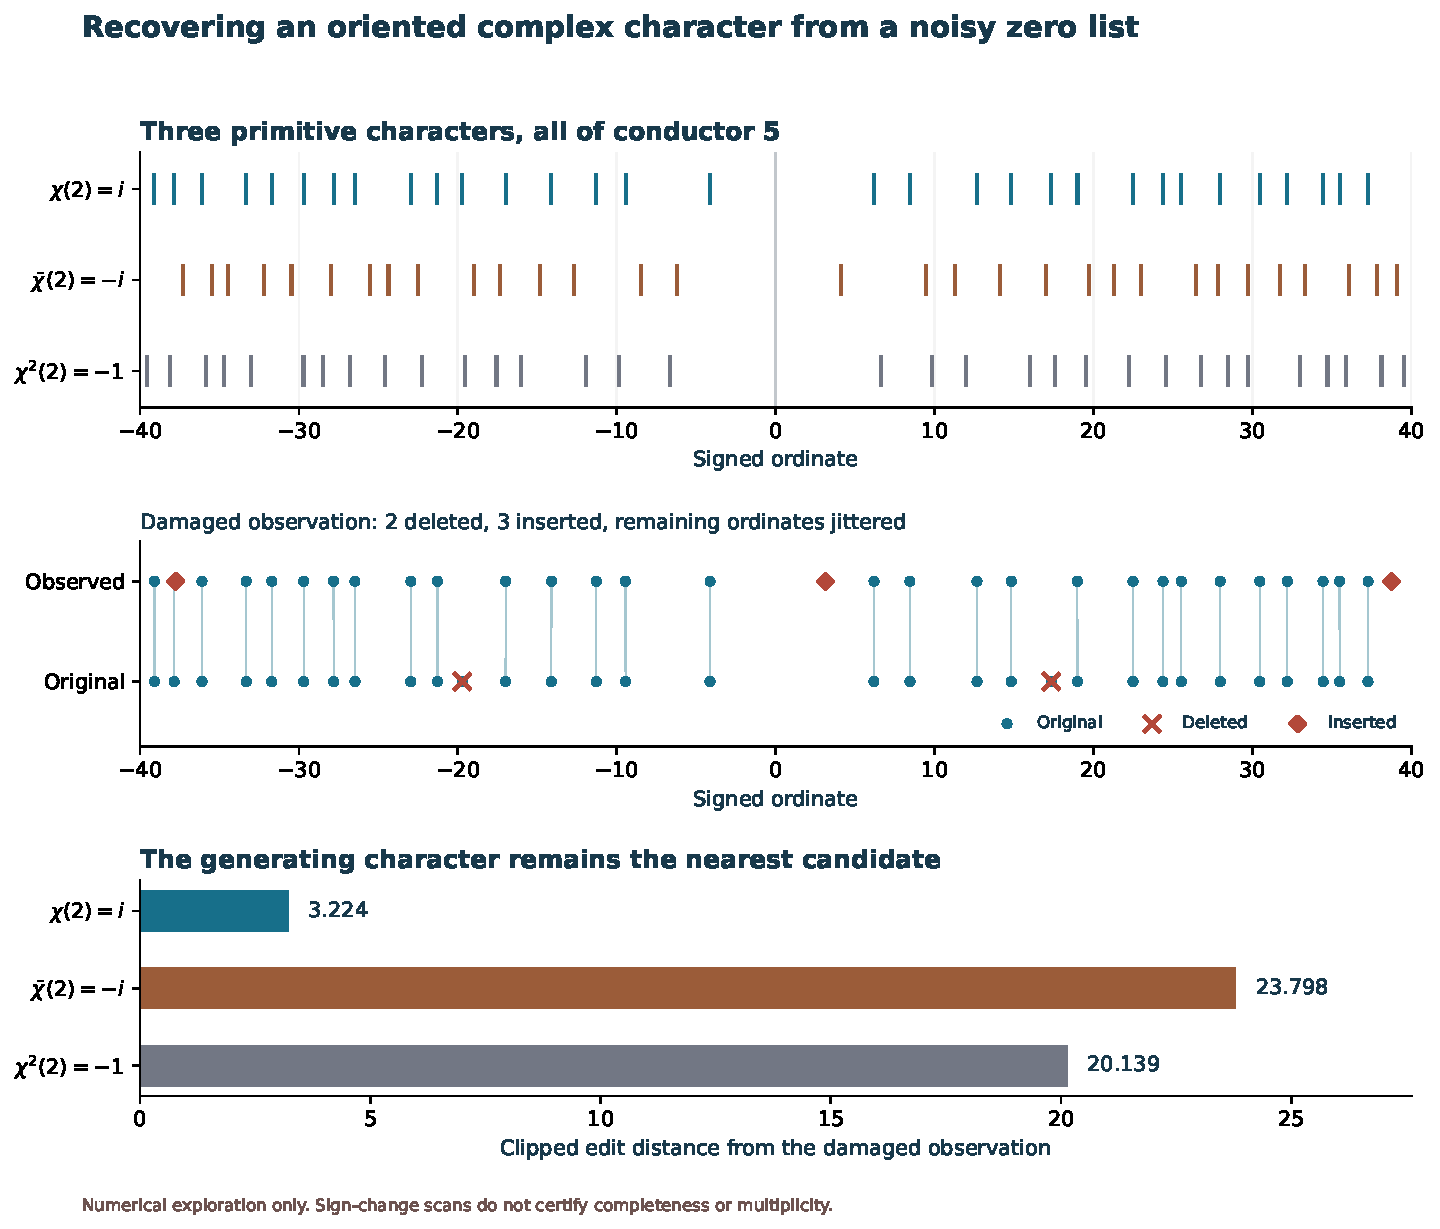
\includegraphics[width=\linewidth]{demo/complex_zero_lists.pdf}
\caption{Signed numerical ordinates for the three conductor-$5$
characters and the damaged observation. The quartic spectrum and
its reflection encode the conjugate orientation. The height-$40$
lists are numerical illustrations, not certified complete spectra.}
\end{figure}

This example is deliberately separated from the theorem's
certificate. A sign-change scan can miss an even-multiplicity zero
or several crossings in one mesh interval. Small residuals verify
the detected approximate roots but do not certify completeness or
multiplicity. Height $40$ is also far below the conservative
universal cutoff in Theorem~\ref{thm:main}. Thus the example
illustrates the observation model and the metric, not an application
of the universal theorem at that height.

\subsection{Checks of the quantitative implementation}

The script \texttt{code/verify\_constants.py} evaluates the specified
cutoff and the explicit tail bound at several conductor bounds,
checks the exact integer inequality $m^2\le3^{m/2}$ for the orders
used in the calculations, and checks the scalar inequalities
appearing in the angular argument. Its output is saved in
\texttt{data/constants.json}. The arguments in the text, rather
than this finite sample of numerical checks, prove the inequalities
over their complete ranges.
